\section{CHAPTER 11: CONTROL AND INSTRUMENTATION}

\subsection{Pressure Control: Pressure reduction -- pneumatic}

\subsubsection{Description}

These control systems may include:

\begin{enumerate}
\item
  P + I + D functions to improve accuracy under varying load conditions.
\item
  Set point(s), which may be remotely adjusted.
\end{enumerate}

\subsubsection{Advantages:}

\begin{enumerate}
\item
  Incredibly precise and adaptable.
\item
  Within the bounds of the valve range, there is no maximum valve size.
\item
  Capable of handling a 50:1 flow range (usually for a globe control
  valve).
\item
  Appropriate for dangerous settings.
\item
  There is no need for an electrical supply.
\item
  Their quick operation allows them to adapt efficiently to sudden
  variations in demand.
\item
  Incredibly strong actuation that can handle large pressure
  differentials across the valve.
\end{enumerate}

\subsubsection{Disadvantages:}

\begin{enumerate}
\item
  More costly than regulations that act on their own.
\item
  More intricate than self-regulating mechanisms.
\item
  Not programmable in a straightforward manner.
\end{enumerate}

\begin{figure}[h!]
  \centering
  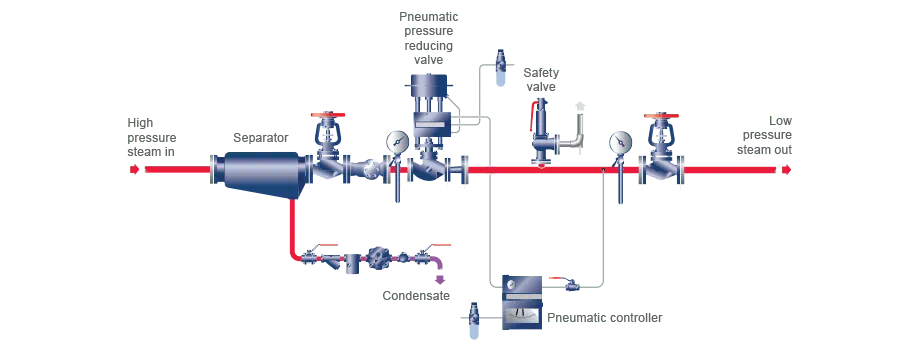
\includegraphics[width=7.01231in,height=2.65972in]{figs/control_instrumentation/image1.png}
  \caption{Pressure reduction system with pneumatic controller.}
  \label{fig:Pressure reduction system with pneumatic controller.}
\end{figure}


\subsection{Pressure reduction -- electro pneumatic}

\subsubsection{Description:}

These control systems may include:

\begin{enumerate}
\item
  P + I + D functions to improve accuracy under varying load conditions.
\item
  Set point(s) which may be remotely adjusted, with the possibility of
  ramps between set points.
\end{enumerate}

\subsubsection{Advantages:}

\begin{enumerate}
\item
  Very precise and adaptable.
\item
  Readout and remote adjustment.
\item
  Within the bounds of the valve range, there is no maximum valve size.
\item
  Capable of handling a 50:1 flow range (usually for a globe control
  valve).
\item
  Quick operation: quick reaction to demand variations.
\item
  Very strong actuation that can handle large pressure differentials
  across the valve.
\end{enumerate}

\subsubsection{Disadvantages:}

\begin{enumerate}
\item
  More costly compared to pneumatic or self-acting controllers.
\item
  More intricate than pneumatic or self-acting controls.
\item
  Requires an electrical control signal. Expensive in dangerous
  locations.
\end{enumerate}

\begin{figure}[h!]
  \centering
  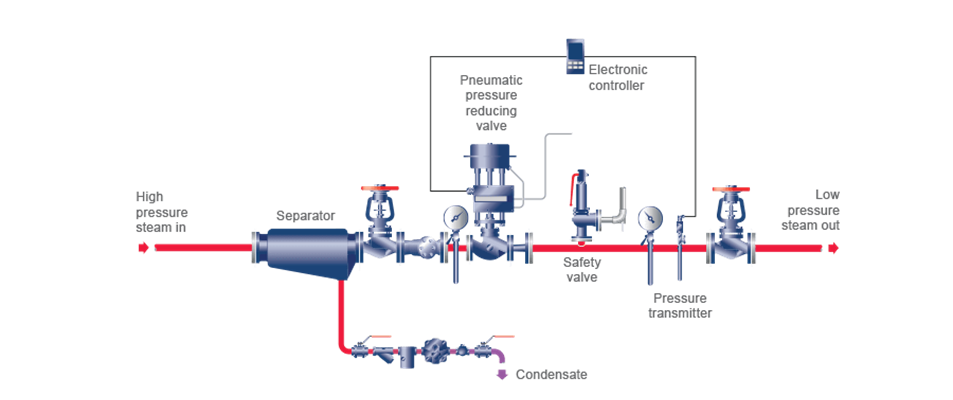
\includegraphics[width=5.60294in,height=2.3514in]{figs/control_instrumentation/image2.png}
  \caption{Pressure reduction system with electro-pneumatic controller.}
  \label{fig:Pressure reduction system with electro-pneumatic controller.}
\end{figure}


\subsection{Pneumatic temperature control}

\subsubsection{Description:}

These control systems may include:

\begin{enumerate}
\item
  P + I + D functions to improve accuracy under varying load conditions.
\item
  Set point(s), which may be remotely adjusted.
\end{enumerate}

\subsubsection{Advantages:}

\begin{enumerate}
\item
  Very precise and adaptable.
\item
  Within the bounds of the valve range, there is no maximum valve size.
\item
  Outstanding ratio of turndowns.
\item
  Appropriate for dangerous settings.
\item
  There is no need for an electrical supply.
\item
  Their quick operation allows them to adapt efficiently to sudden
  variations in demand.
\item
  Very strong and resilient to large differential pressures.
\end{enumerate}

\subsubsection{Disadvantages:}

\begin{enumerate}
\item
  Costlier than running controls that are direct.
\item
  More intricate than simple operational controls.
\end{enumerate}

\begin{figure}[h!]
  \centering
  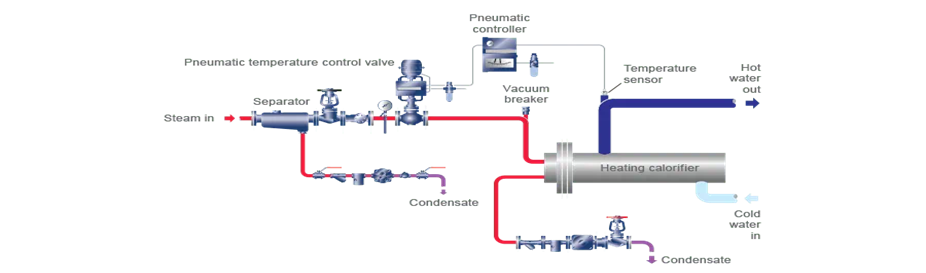
\includegraphics[width=6.14961in,height=2.16177in]{figs/control_instrumentation/image3.png}
  \caption{Temperature (pneumatic) controller}
  \label{fig:Temperature (pneumatic) controller}
\end{figure}


\subsection{Electro pneumatic temperature control}

\subsubsection{Description}

These control systems may include:

\begin{enumerate}
\item
  P + I + D functions to improve accuracy under varying load conditions.
\item
  Set point(s) may be remotely adjusted, with the possibility of ramps
  between set points.
\end{enumerate}

\subsubsection{Advantages:}

\begin{enumerate}
\item
  Very precise and adaptable.
\item
  Readout and remote adjustment.
\item
  Within the bounds of the valve range, there is no maximum valve size.
\item
  Outstanding ratio of turndowns.
\item
  Their quick operation allows them to adapt efficiently to sudden
  variations in demand.
\item
  Very strong and resilient to large differential pressures.
\end{enumerate}

\subsubsection{Disadvantages:}

\begin{enumerate}
\item
  More costly compared to pneumatic or self-acting controllers.
\item
  More intricate than pneumatic or self-acting controls.
\item
An electrical source is necessary.
\end{enumerate}

\begin{figure}[h!]
  \centering
  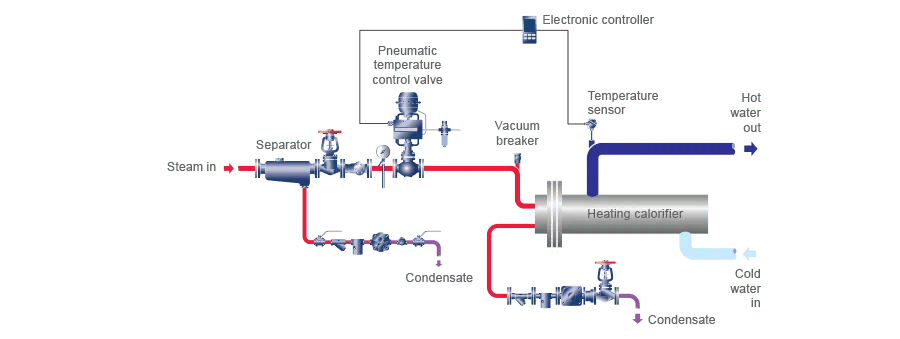
\includegraphics[width=5.88235in,height=1.95588in]{figs/control_instrumentation/image4.png}
  \caption{Electro-pneumatic temperature controller}
  \label{fig:Electro-pneumatic temperature controller}
\end{figure}



\subsection{Level Control}

Adjustable on/off level control

\subsubsection{Description}

An adjustable on/off level control system consists of a controller and a
capacitance probe (see Figure 3.32), and provides:

\begin{enumerate}
\item
  One alarm point in addition to an open/closed valve control.
\item
  As an alternative, set a low and a high alarm.
\item
  The controller functions allow for the adjustment of the
  valve\textquotesingle s operating levels.
\end{enumerate}

\subsubsection{Advantage:}

\begin{enumerate}
\item
  The operation may be stopped without changing the level settings
  thanks to the adjustable on/off level control.
\end{enumerate}

\subsubsection{Disadvantage:}

\begin{enumerate}
\item
  More costly than an on/off switch that isn\textquotesingle t
  changeable.
\item
  Applications: Suitable for a wide range of liquids, including those
  with poor conductivities.
\item
Noteworthy:  It may be utilised in conditions when the liquid surface is turbulent,
and the built-in electronics can be modified to stop the pump (or
valve) from cycling rapidly on and off.
\end{enumerate}

\begin{figure}[h!]
  \centering
  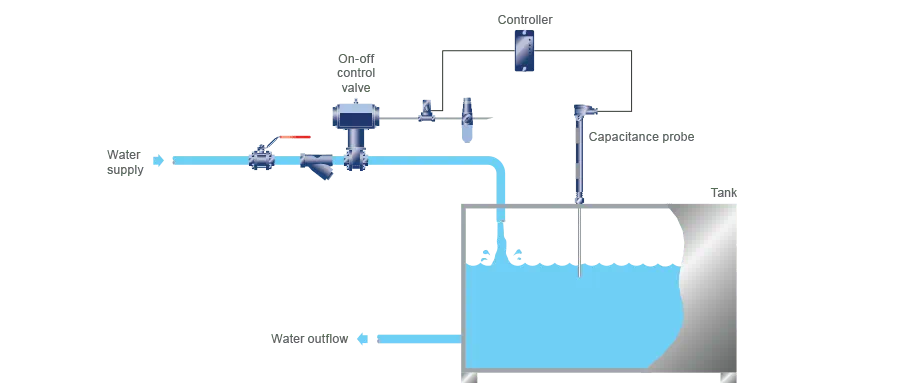
\includegraphics[width=6.75312in,height=3in]{figs/control_instrumentation/image5.png}
  \caption{On/off level controller}
  \label{fig:On/off level controller}
\end{figure}


\subsection{Modulating level control}

\subsubsection{Description:}

A capacitance probe and suitable controller, which generates a
modulating output signal, usually 4--20 mA, make up a modulating level
control system. See Figure 8.3.5. Several devices may be impacted by
this output signal, including:

\begin{enumerate}
\item
  Modulating a control valve.
\item
  Operating a variable speed pump drive.
\end{enumerate}

\subsubsection{Advantage:}

\begin{enumerate}
\item
  The scale of the application is unlimited as the probe and controller
  don\textquotesingle t really supply the power to run a
  device---rather, they only send out a signal that other devices react
  to.
\item
  Steady regulation of the tank\textquotesingle s level.
\end{enumerate}

\subsubsection{Disadvantage:}

\begin{enumerate}
\item
  More expensive than a conductivity probe system.
\item
  More complex than a conductivity probe system.
\item
  Supply system must be permanently charged.
\item
  Less suitable for `stand-by' operation.
\item
  Possibly greater electricity consumption.
\end{enumerate}


\begin{figure}[h!]
  \centering
  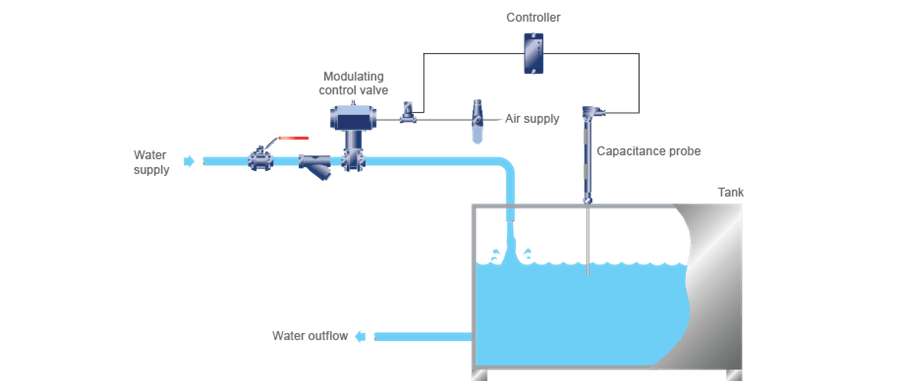
\includegraphics[width=6in,height=2.65278in]{figs/control_instrumentation/image6.png}
  \caption{Modulating level controller}
  \label{fig:Modulating level controller}
\end{figure}



\subsection{Desuperheaters}

Desuperheating is the process of lowering the superheated temperature of
steam or returning it to its saturated condition. A direct contact type
pipeline desuperheater and a pressure lowering station are arranged in
the system shown in Figure 3.34.



In its simplest form, high-quality water, usually condensate, is injected
into the flow of superheated steam, which removes heat and lowers the
temperature of the steam. Because the control system cannot distinguish
between saturated and wet steam at the same temperature, it is not
practicable to lower the steam temperature to its saturated value. As a
result, the temperature is constantly maintained at a level that is
greater than the applicable saturation temperature, often between 5 and
10 degrees Celsius above saturation.

\begin{figure}[h!]
  \centering
  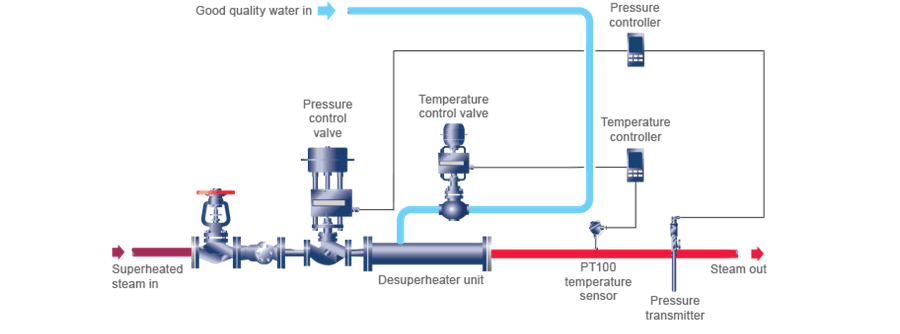
\includegraphics[width=0.7\linewidth]{figs/control_instrumentation/image7.png}
  \caption{Desuperheating unit.}
  \label{fig:Desuperheating unit}
\end{figure}


This illustrates a simple setup that will function well for most
purposes. The set setting on the temperature controller only has to be
set slightly above the matching saturation temperature since the
pressure control loop maintains the downstream pressure at a constant
value.

If the downstream pressure fluctuates, as it sometimes does with certain
industrial operations, a modification in the water/steam flow ratio will
also be necessary.

The steam pressure control valve in the system shown in Figure 3.34 is
operated by setting the pressure controller to the necessary downstream
pressure.

The pressure transmitter\textquotesingle s 4--20 mA signal is sent to
the saturation temperature computer and pressure controller. The
computer uses this information to continuously determine the downstream
pressure\textquotesingle s saturation temperature and sends a 4--20 mA
output signal to the temperature controller based on that temperature.

The temperature controller is set up to detect its set point at 5°C to
10°C above saturation by accepting a 4--20 mA signal from the computer.
In this manner, the temperature set point will automatically change if
the downstream pressure changes for any of the previously listed causes.
This will ensure that, regardless of load or downstream pressure, the
proper ratio of water to steam is maintained.


\subsection{PID Controller:}

One popular kind of feedback control system in industrial control
systems is the PID controller. Proportional-Integral-Derivative, or PID,
is the acronym for the three words used to modify the control signal
sent to the system:

\textbf{Proportional (P):} The output value generated by this term is
proportionate to the error value that is now present. It responds to the
current mistake. By multiplying the error by a constant called the
proportional gain (Kp), one may modify the proportional response. The
system may respond violently when the Kp is high, but a Kp that is too
high may induce instability.

\textbf{Integral (I):} The accumulation of previous mistakes is the
subject of this word. The integral term accumulates the mistake if it
continues over time, and this accumulation is amplified by the integral
gain (Ki). It assists in removing steady-state error residue that the
proportional term is unable to remove.

\textbf{Derivative (D):} This term uses its rate of change to anticipate
future inaccuracy. It is modified by the derivative gain (Kd) and
responds to the rate at which the error is changing. The derivative term
contributes to increased stability by reducing overshoot and damping
down the system response.

\begin{figure}[h!]
  \centering
  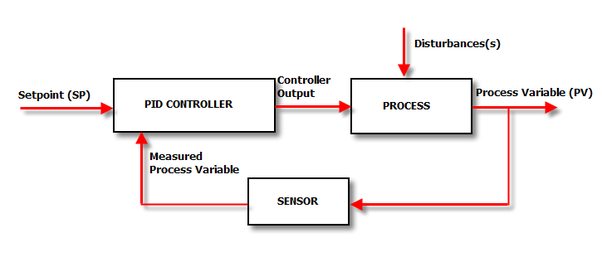
\includegraphics[width=0.7\linewidth]{figs/control_instrumentation/image8.png}
  \caption{Work flow diagram of PID controller}
  \label{fig:Work flow diagram of PID controller}
\end{figure}

\subsection{Programmable Logic Controller (PLC)}

\textbf{Definition:} A PLC is an industrial digital computer that is
used to manage robotic devices, assembly lines, and other production
processes that need to be highly dependable and simple to program.

\textbf{Key Features:}

\begin{enumerate}
\item
  Robust and robust: Designed to endure challenging industrial settings.
\item
  Real-time operation: Able to react in real-time to changes in input.
\item
  Programmable: Makes use of structured text, ladder logic, and function
  block diagrams, among other programming languages.
\item
  I/O Modules: Actuator and sensor interfaces.
\end{enumerate}

\textbf{Applications:} Used in automation of machinery on factory
assembly lines, amusement rides, light fixtures, and more.


\begin{figure}[h!]
  \centering 
  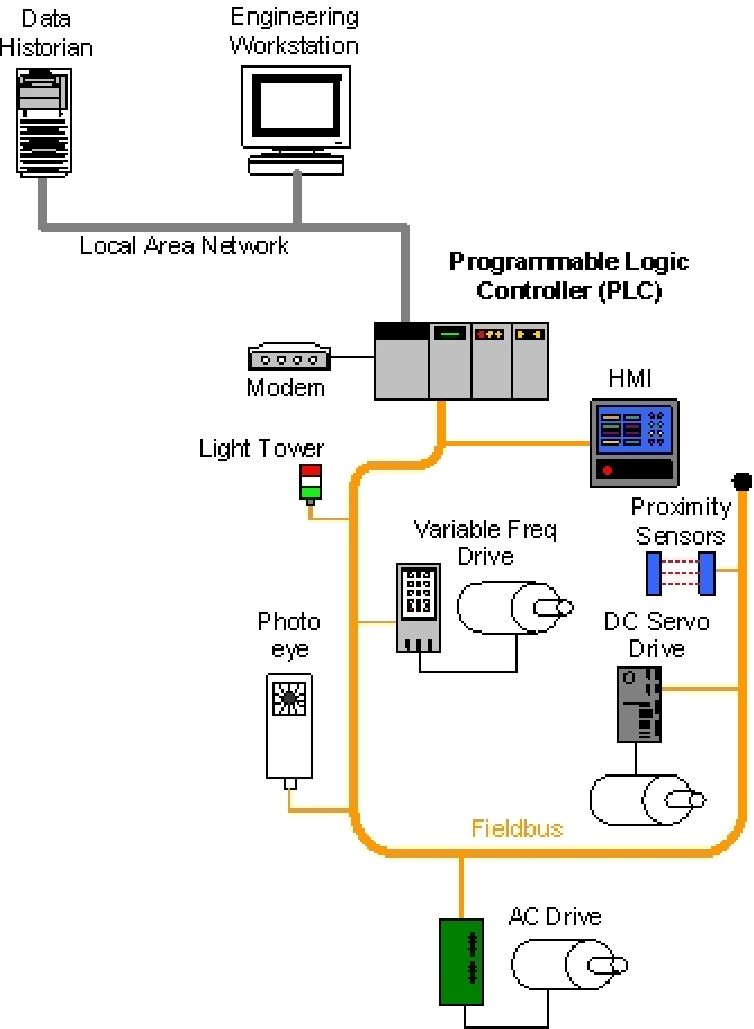
\includegraphics[width=1.97887in,height=2.18448in]{figs/control_instrumentation/image9.png}
  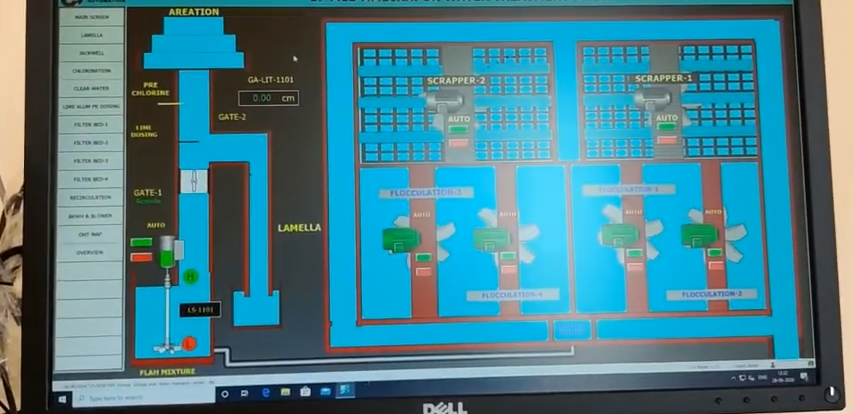
\includegraphics[width=3.96887in,height=2.08876in]{figs/control_instrumentation/image10.png}
  \caption{SCADA system for water level control}
  \label{fig:SCADA system for water level control}
\end{figure}


\subsection{Supervisory Control and Data Acquisition (SCADA)}

\textbf{Definition:} SCADA is a control system architecture that
provides high-level process supervisory management via the use of
computers, networked data transmission, and graphical user interfaces.

\textbf{Key Features:}

\begin{enumerate}
\item
  Monitoring, obtaining, and processing real-time data is known as
  real-time data collection.
\item
  Remote control: Offers process monitoring and control from a distance.
\item
  Alarms and data logging: Records data for analysis and sounds an alert
  when certain criteria are met.
\item
  Graphical user interface used by operators to communicate with the
  system is known as the Human-Machine Interface (HMI).
\end{enumerate}

\textbf{Applications:} Used in various industries like water treatment
plants, oil and gas pipelines, power generation, and distribution.

\subsection{Distributed Control System (DCS)}

\textbf{Definition:} A distributed control system (DCS) is a process or
plant control system in which the control components are dispersed
throughout the system instead of being centralized at a single point.

\textbf{Key Features:}

\begin{enumerate}
\item
  Decentralized control: Every area of the plant has a controller that
  connects to other controllers via communication.
\item
  Scalability: Large and sophisticated operations can be easily scaled.
\item
  Integration: For higher-level monitoring, integrates often with other
  systems, including SCADA.
\item
  System dependability is increased by having redundant communication
  channels and controllers.
\end{enumerate}

\textbf{Applications:} Commonly used in large-scale industrial processes
such as chemical plants, oil refineries, and power stations where
continuous and complex operations are required.




\begin{figure}[h!]
  \centering
  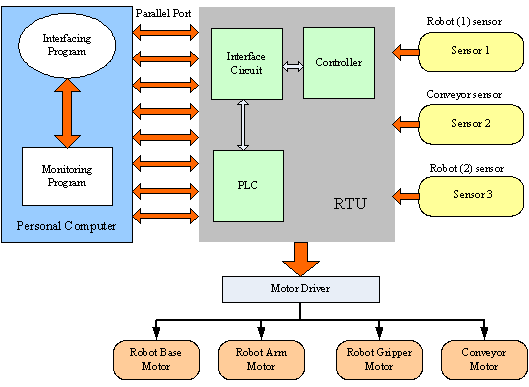
\includegraphics[width=2.704in,height=1.97862in]{figs/control_instrumentation/image11.png}
  \caption{Block diagram of DCS for manufacturing plant.}
  \label{fig:Block diagram of DCS}
\end{figure}